\documentclass{standalone}
\usepackage{tikz}
\usetikzlibrary{patterns, positioning}


\begin{document}
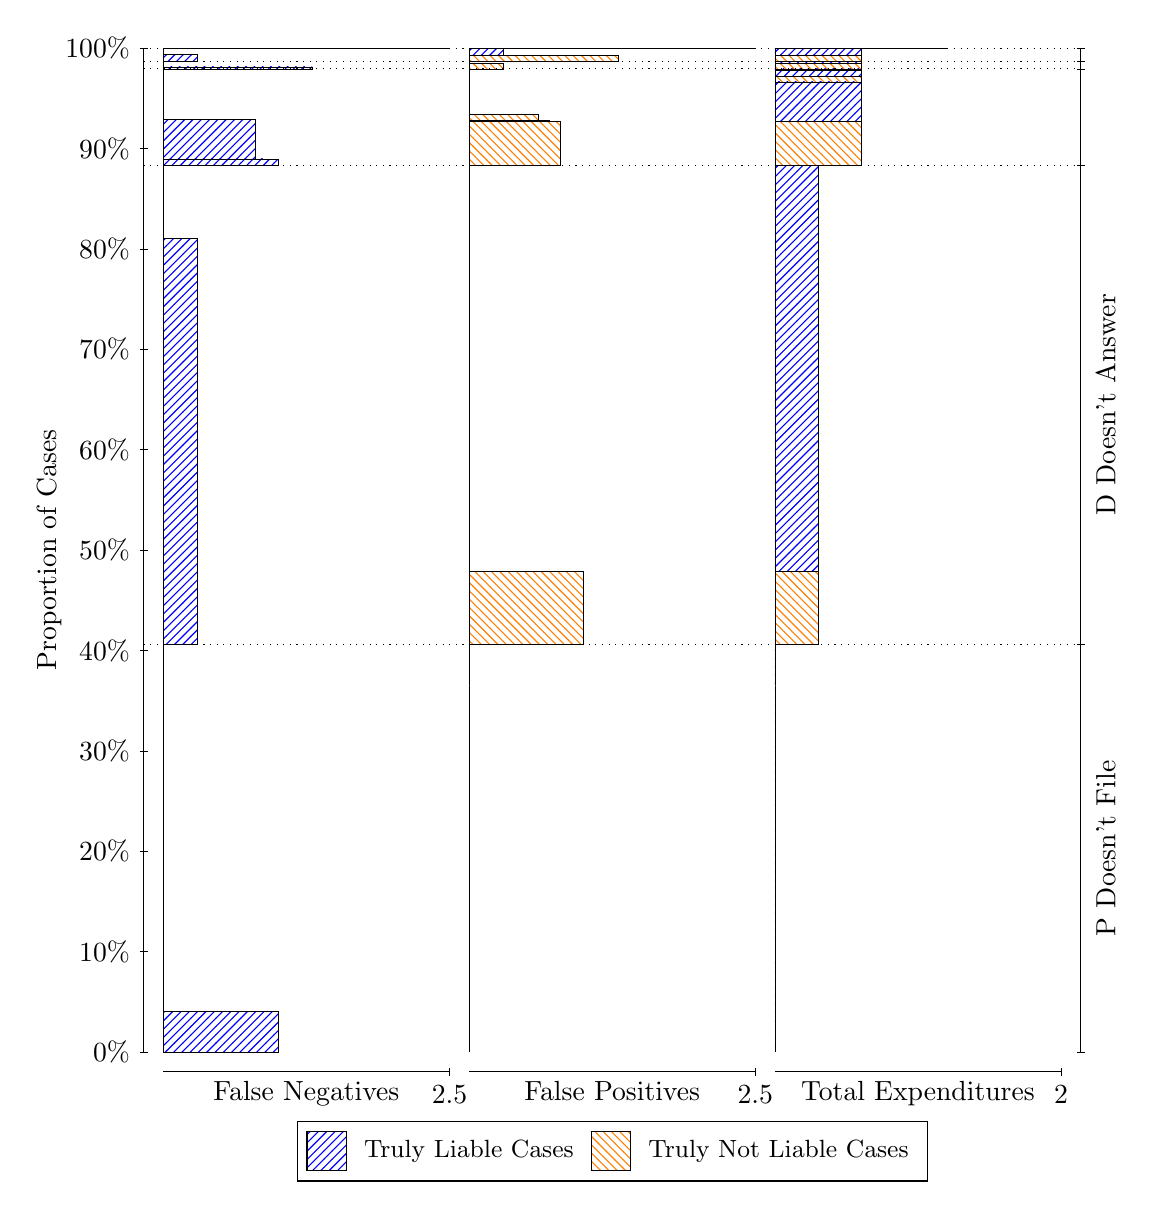
\begin{tikzpicture}
\draw[black, very thin] (1.5,1.75) -- (1.5,14.5);
\node[rotate=90, text=black, anchor=center] at (0.3, 8.125) {Proportion of Cases};
\draw[black, very thin] (1.45,1.75) -- (1.55,1.75);
\node[text=black, anchor=east] at (1.45, 1.75) {0\%};
\draw[black, very thin] (1.45,3.025) -- (1.55,3.025);
\node[text=black, anchor=east] at (1.45, 3.025) {10\%};
\draw[black, very thin] (1.45,4.3) -- (1.55,4.3);
\node[text=black, anchor=east] at (1.45, 4.3) {20\%};
\draw[black, very thin] (1.45,5.575) -- (1.55,5.575);
\node[text=black, anchor=east] at (1.45, 5.575) {30\%};
\draw[black, very thin] (1.45,6.85) -- (1.55,6.85);
\node[text=black, anchor=east] at (1.45, 6.85) {40\%};
\draw[black, very thin] (1.45,8.125) -- (1.55,8.125);
\node[text=black, anchor=east] at (1.45, 8.125) {50\%};
\draw[black, very thin] (1.45,9.4) -- (1.55,9.4);
\node[text=black, anchor=east] at (1.45, 9.4) {60\%};
\draw[black, very thin] (1.45,10.675) -- (1.55,10.675);
\node[text=black, anchor=east] at (1.45, 10.675) {70\%};
\draw[black, very thin] (1.45,11.95) -- (1.55,11.95);
\node[text=black, anchor=east] at (1.45, 11.95) {80\%};
\draw[black, very thin] (1.45,13.225) -- (1.55,13.225);
\node[text=black, anchor=east] at (1.45, 13.225) {90\%};
\draw[black, very thin] (1.45,14.5) -- (1.55,14.5);
\node[text=black, anchor=east] at (1.45, 14.5) {100\%};

\draw[black, very thin] (13.4,1.75) -- (13.4,14.5);
\draw[black, very thin] (13.35,1.75) -- (13.45,1.75);
\node[anchor=west] at (13.35, 1.75) {};
\draw[black, very thin] (13.35,6.9249) -- (13.45,6.9249);
\node[anchor=west] at (13.35, 6.9249) {};
\draw[black, very thin] (13.35,13.012) -- (13.45,13.012);
\node[anchor=west] at (13.35, 13.012) {};
\draw[black, very thin] (13.35,14.236) -- (13.45,14.236);
\node[anchor=west] at (13.35, 14.236) {};
\draw[black, very thin] (13.35,14.333) -- (13.45,14.333);
\node[anchor=west] at (13.35, 14.333) {};
\draw[black, very thin] (13.35,14.494) -- (13.45,14.494);
\node[anchor=west] at (13.35, 14.494) {};
\draw[black, very thin] (13.35,14.498) -- (13.45,14.498);
\node[anchor=west] at (13.35, 14.498) {};
\draw[black, very thin] (13.35,14.5) -- (13.45,14.5);
\node[anchor=west] at (13.35, 14.5) {};

\draw[black, very thin, pattern color=blue, pattern=north east lines] (1.75,1.75) rectangle (3.2033,2.2693);
\draw[black, very thin, pattern color=orange, pattern=north west lines] (1.75,2.2693) rectangle (1.75,6.9249);
\draw[black, very thin, pattern color=blue, pattern=north east lines] (1.75,6.9249) rectangle (2.186,12.084);
\draw[black, very thin, pattern color=orange, pattern=north west lines] (1.75,12.084) rectangle (1.75,13.012);
\draw[black, very thin, pattern color=blue, pattern=north east lines] (1.75,13.012) rectangle (3.2033,13.084);
\draw[black, very thin, pattern color=blue, pattern=north east lines] (1.75,13.084) rectangle (3.058,13.091);
\draw[black, very thin, pattern color=blue, pattern=north east lines] (1.75,13.091) rectangle (2.9127,13.592);
\draw[black, very thin, pattern color=orange, pattern=north west lines] (1.75,13.592) rectangle (1.75,14.236);
\draw[black, very thin, pattern color=blue, pattern=north east lines] (1.75,14.236) rectangle (3.6393,14.261);
\draw[black, very thin, pattern color=orange, pattern=north west lines] (1.75,14.261) rectangle (1.75,14.333);
\draw[black, very thin, pattern color=blue, pattern=north east lines] (1.75,14.333) rectangle (2.186,14.422);
\draw[black, very thin, pattern color=orange, pattern=north west lines] (1.75,14.422) rectangle (1.75,14.494);
\draw[black, very thin, pattern color=blue, pattern=north east lines] (1.75,14.494) rectangle (5.3833,14.495);
\draw[black, very thin, pattern color=orange, pattern=north west lines] (1.75,14.495) rectangle (1.75,14.498);
\draw[black, very thin, pattern color=orange, pattern=north west lines] (1.75,14.498) rectangle (1.75,14.499);
\draw[black, very thin, pattern color=blue, pattern=north east lines] (1.75,14.499) rectangle (1.75,14.5);
\draw[black, very thin, pattern color=orange, pattern=north west lines] (5.6333,1.75) rectangle (5.6333,6.4055);
\draw[black, very thin, pattern color=blue, pattern=north east lines] (5.6333,6.4055) rectangle (5.6333,6.9249);
\draw[black, very thin, pattern color=orange, pattern=north west lines] (5.6333,6.9249) rectangle (7.0867,7.8527);
\draw[black, very thin, pattern color=blue, pattern=north east lines] (5.6333,7.8527) rectangle (5.6333,13.012);
\draw[black, very thin, pattern color=orange, pattern=north west lines] (5.6333,13.012) rectangle (6.796,13.568);
\draw[black, very thin, pattern color=orange, pattern=north west lines] (5.6333,13.568) rectangle (6.6507,13.584);
\draw[black, very thin, pattern color=orange, pattern=north west lines] (5.6333,13.584) rectangle (6.5053,13.656);
\draw[black, very thin, pattern color=blue, pattern=north east lines] (5.6333,13.656) rectangle (5.6333,14.236);
\draw[black, very thin, pattern color=orange, pattern=north west lines] (5.6333,14.236) rectangle (6.0693,14.308);
\draw[black, very thin, pattern color=blue, pattern=north east lines] (5.6333,14.308) rectangle (5.6333,14.333);
\draw[black, very thin, pattern color=orange, pattern=north west lines] (5.6333,14.333) rectangle (7.5227,14.405);
\draw[black, very thin, pattern color=blue, pattern=north east lines] (5.6333,14.405) rectangle (6.0693,14.494);
\draw[black, very thin, pattern color=orange, pattern=north west lines] (5.6333,14.494) rectangle (5.6333,14.497);
\draw[black, very thin, pattern color=blue, pattern=north east lines] (5.6333,14.497) rectangle (5.6333,14.498);
\draw[black, very thin, pattern color=orange, pattern=north west lines] (5.6333,14.498) rectangle (9.2667,14.499);
\draw[black, very thin, pattern color=blue, pattern=north east lines] (5.6333,14.499) rectangle (7.8133,14.5);
\draw[black, very thin, pattern color=orange, pattern=north west lines] (9.5167,1.75) rectangle (9.5167,6.4055);
\draw[black, very thin, pattern color=blue, pattern=north east lines] (9.5167,6.4055) rectangle (9.5167,6.9249);
\draw[black, very thin, pattern color=orange, pattern=north west lines] (9.5167,6.9249) rectangle (10.062,7.8527);
\draw[black, very thin, pattern color=blue, pattern=north east lines] (9.5167,7.8527) rectangle (10.062,13.012);
\draw[black, very thin, pattern color=orange, pattern=north west lines] (9.5167,13.012) rectangle (10.607,13.568);
\draw[black, very thin, pattern color=blue, pattern=north east lines] (9.5167,13.568) rectangle (10.607,14.069);
\draw[black, very thin, pattern color=orange, pattern=north west lines] (9.5167,14.069) rectangle (10.607,14.141);
\draw[black, very thin, pattern color=blue, pattern=north east lines] (9.5167,14.141) rectangle (10.607,14.213);
\draw[black, very thin, pattern color=orange, pattern=north west lines] (9.5167,14.213) rectangle (10.607,14.229);
\draw[black, very thin, pattern color=blue, pattern=north east lines] (9.5167,14.229) rectangle (10.607,14.236);
\draw[black, very thin, pattern color=orange, pattern=north west lines] (9.5167,14.236) rectangle (10.607,14.308);
\draw[black, very thin, pattern color=blue, pattern=north east lines] (9.5167,14.308) rectangle (10.607,14.333);
\draw[black, very thin, pattern color=orange, pattern=north west lines] (9.5167,14.333) rectangle (10.607,14.405);
\draw[black, very thin, pattern color=blue, pattern=north east lines] (9.5167,14.405) rectangle (10.607,14.494);
\draw[black, very thin, pattern color=orange, pattern=north west lines] (9.5167,14.494) rectangle (11.697,14.497);
\draw[black, very thin, pattern color=blue, pattern=north east lines] (9.5167,14.497) rectangle (11.697,14.498);
\draw[black, very thin, pattern color=orange, pattern=north west lines] (9.5167,14.498) rectangle (11.697,14.499);
\draw[black, very thin, pattern color=blue, pattern=north east lines] (9.5167,14.499) rectangle (11.697,14.5);
\draw[black, dotted] (1.5,6.9249) -- (13.4,6.9249);
\draw[black, dotted] (1.5,13.012) -- (13.4,13.012);
\draw[black, dotted] (1.5,14.236) -- (13.4,14.236);
\draw[black, dotted] (1.5,14.333) -- (13.4,14.333);
\draw[black, dotted] (1.5,14.494) -- (13.4,14.494);
\draw[black, dotted] (1.5,14.498) -- (13.4,14.498);
\draw[black, very thin] (1.75,1.5) -- (5.3833,1.5);
\node[text=black, anchor=north] at (3.5667, 1.5) {False Negatives};
\draw[black, very thin] (5.3833,1.45) -- (5.3833,1.55);
\node[text=black, anchor=north] at (5.3833, 1.45) {2.5};

\draw[black, very thin] (5.6333,1.5) -- (9.2667,1.5);
\node[text=black, anchor=north] at (7.45, 1.5) {False Positives};
\draw[black, very thin] (9.2667,1.45) -- (9.2667,1.55);
\node[text=black, anchor=north] at (9.2667, 1.45) {2.5};

\draw[black, very thin] (9.5167,1.5) -- (13.15,1.5);
\node[text=black, anchor=north] at (11.333, 1.5) {Total Expenditures};
\draw[black, very thin] (13.15,1.45) -- (13.15,1.55);
\node[text=black, anchor=north] at (13.15, 1.45) {2};

\node[text=black, centered, rotate=90] at (13.72, 4.3374) {P Doesn't File};
\node[text=black, centered, rotate=90] at (13.72, 9.9684) {D Doesn't Answer};






\draw (7.449999999999999,1.5) node[draw=none] (baseCoordinate) {};
\begin{scope}[align=center]
        \matrix[scale=0.5, draw=black, below=0.5cm of baseCoordinate, nodes={draw}, column sep=0.1cm]{
            \node[rectangle, draw, minimum width=0.5cm, minimum height=0.5cm, pattern color=blue, pattern=north east lines] {}; &
            \node[draw=none, font=\small, text=black] (B) {Truly Liable Cases}; &
            \node[rectangle, draw, minimum width=0.5cm, minimum height=0.5cm, pattern color=orange, pattern=north west lines] {}; &
            \node[draw=none, font=\small, text=black] (B) {Truly Not Liable Cases}; \\
            };
\end{scope}

\end{tikzpicture}
\end{document}